%--------------------------------------------CAPA MOTIACIONAL ------------------------------------------------------%


\subsection{Capa motivacional}

Los elementos de motivación se utilizan para modelar las motivaciones o \textbf{razones que guían el diseño o cambio de una arquitectura empresarial.}

La tabla \ref{tab:Tabla de la capa de motivación} ofrece una visión general de los elementos de motivación, con sus definiciones. \cite{archimate}

\begin{longtable}{|p{0.15\linewidth}|p{0.45\linewidth}|p{0.2\linewidth} p{0.2\linewidth}|}
    \caption{Tabla de la capa de motivación}
    \\
    \hline
    \rowcolor[HTML]{DAE8FC} 
    \textbf{Elemento} & \textbf{Definición} & \multicolumn{2}{c|}{\textbf{Notación}} \\
    \hline
    \endhead
    \hline
    \multicolumn{4}{r}{\textit{Continúa en la siguiente página}} \\
    \endfoot
    \hline
    \endlastfoot
    \label{tab:Tabla de la capa de motivación}
    %Contenido 1 &
    %\lipsum[1] &
    %Datos A1
    %& Datos B1
    %\\
    %\hline

    Interesado &
    Representa el papel de un individuo, equipo u organización (o clases de ellos) que representa sus intereses en los efectos de la arquitectura. &
\begin{center}
    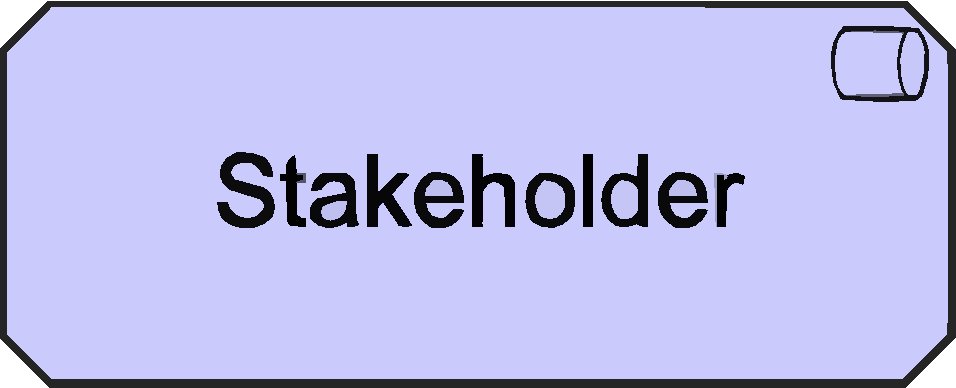
\includegraphics[width=1\linewidth]{imgs/capa_motivacional/stakeholder1.pdf}
\end{center} &
\begin{center}
    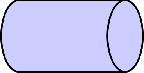
\includegraphics[width=0.7\linewidth]{imgs/capa_motivacional/stakeholder2.pdf}
\end{center}
    \\ \hline

    Conductor &
    Representa una condición externa o interna que motiva a una organización a definir sus objetivos e implementar los cambios necesarios para alcanzarlos. &
\begin{center}
    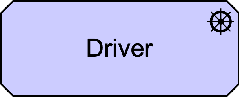
\includegraphics[width=1\linewidth]{imgs/capa_motivacional/driver1.pdf}
\end{center} &
\begin{center}
    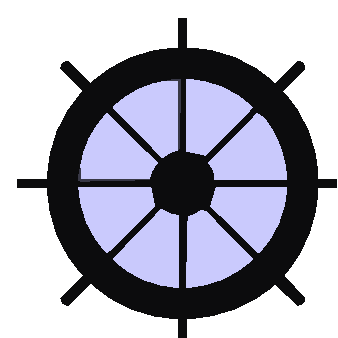
\includegraphics[width=0.5\linewidth]{imgs/capa_motivacional/driver2.pdf}
\end{center}
    \\ \hline

    Evaluación &
    Representa el resultado de un análisis del estado de cosas de la empresa con respecto a algún conductor. &
\begin{center}
    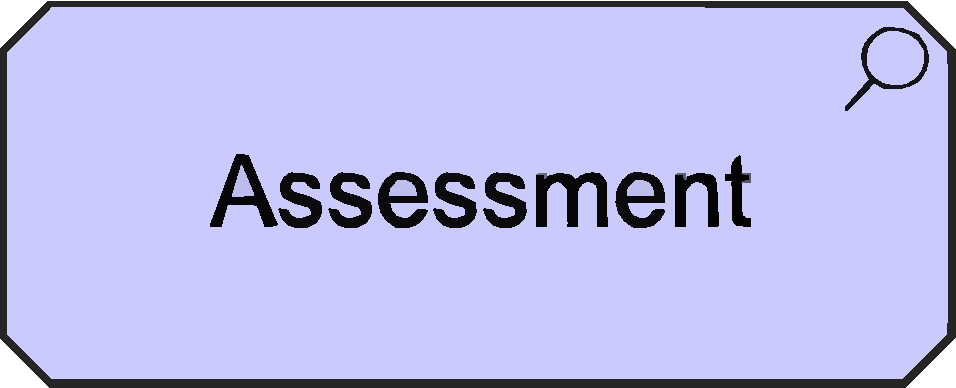
\includegraphics[width=1\linewidth]{imgs/capa_motivacional/assessment1.pdf}
\end{center} &
\begin{center}
    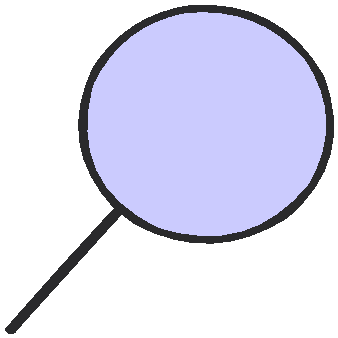
\includegraphics[width=0.5\linewidth]{imgs/capa_motivacional/assessment2.pdf}
\end{center}
    \\ \hline

    Meta &
    Representa una declaración de intención, dirección o estado final deseado de alto nivel para una organización y sus partes interesadas. &
\begin{center}
    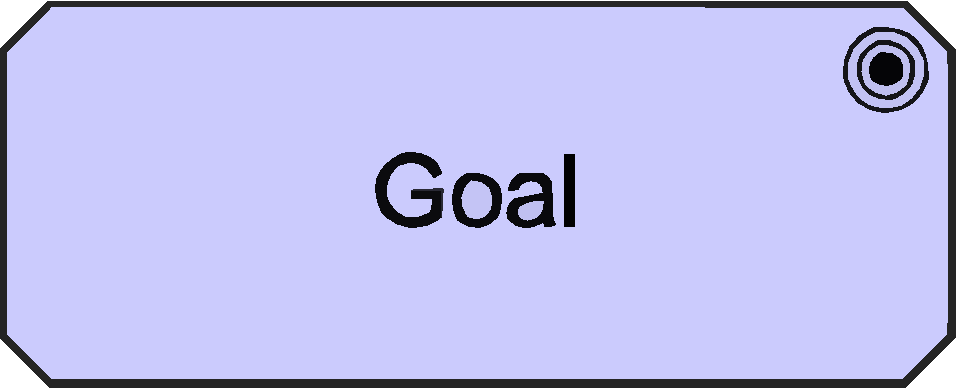
\includegraphics[width=1\linewidth]{imgs/capa_motivacional/goal1.pdf}
\end{center} &
\begin{center}
    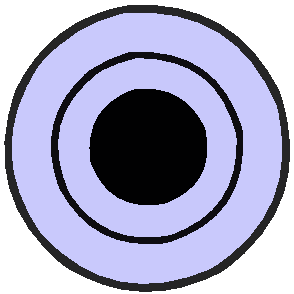
\includegraphics[width=0.5\linewidth]{imgs/capa_motivacional/goal2.pdf}
\end{center}
    \\ \hline

    Resultado &
    Representa un resultado final, efecto o consecuencia de un determinado estado de cosas. &
\begin{center}
    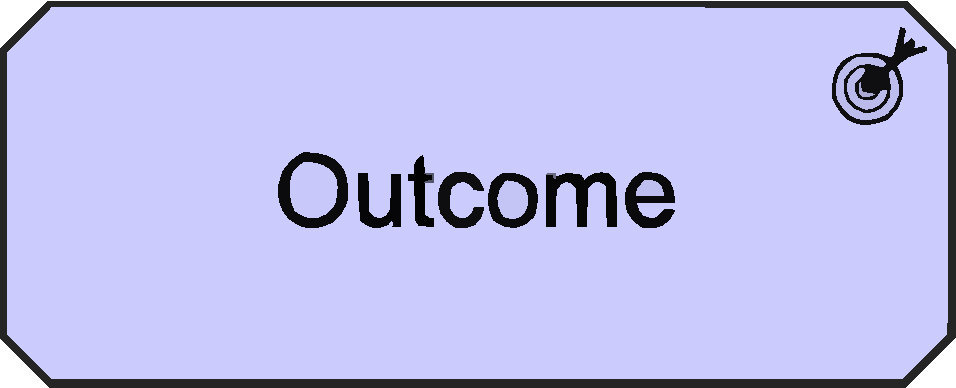
\includegraphics[width=1\linewidth]{imgs/capa_motivacional/outcome1.pdf}
\end{center} &
\begin{center}
    
\includegraphics[width=0.5\linewidth]{imgs/capa_motivacional/outcome2.pdf}
\end{center}
    \\ \hline

    Principio &
    Representa una declaración de intenciones que define una propiedad general que se aplica a cualquier sistema en un contexto determinado de la arquitectura. &
\begin{center}
    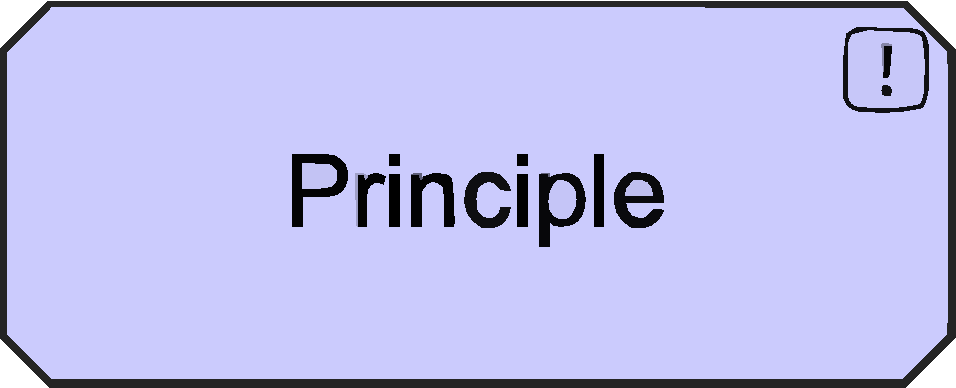
\includegraphics[width=1\linewidth]{imgs/capa_motivacional/principle1.pdf}
\end{center} &
\begin{center}
    
\includegraphics[width=0.5\linewidth]{imgs/capa_motivacional/principle2.pdf}
\end{center}
    \\ \hline

    Requisito &
    Representa una declaración de necesidad que define una propiedad que se aplica a un sistema específico según lo descrito por la arquitectura. &
\begin{center}
    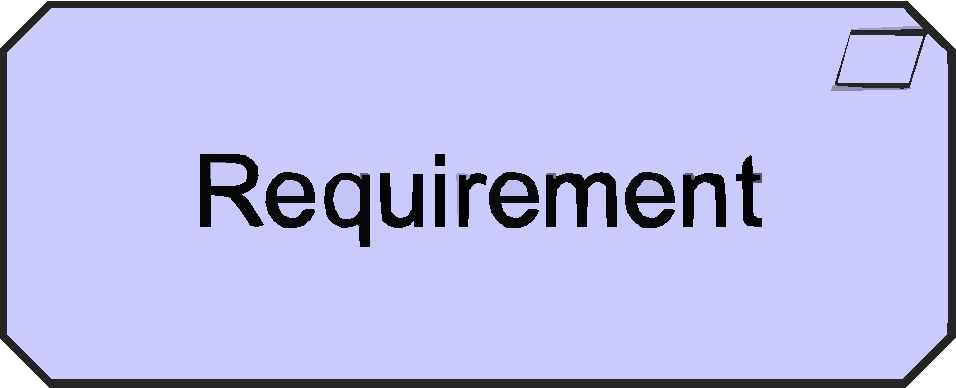
\includegraphics[width=1\linewidth]{imgs/capa_motivacional/requirement1.pdf}
\end{center} &
\begin{center}
    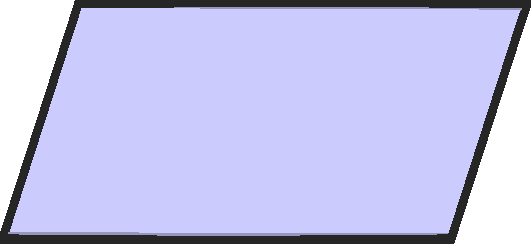
\includegraphics[width=0.5\linewidth]{imgs/capa_motivacional/requirement2.pdf}
\end{center}
    \\ \hline

    Restricción &
    Representa una limitación sobre aspectos de la arquitectura, su proceso de implementación o su realización. &
\begin{center}
    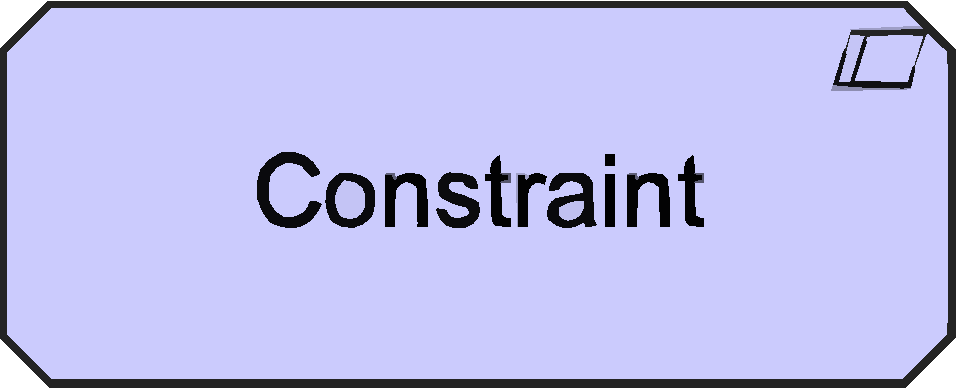
\includegraphics[width=1\linewidth]{imgs/capa_motivacional/constraint1.pdf}
\end{center} &
\begin{center}
    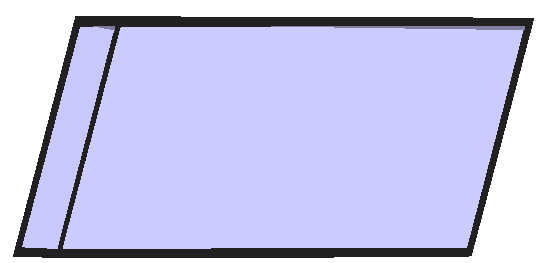
\includegraphics[width=0.5\linewidth]{imgs/capa_motivacional/constraint2.pdf}
\end{center}
    \\ \hline

    Significado &
    Representa el conocimiento o experiencia presente en, o la interpretación dada a, un concepto en un contexto particular. &
\begin{center}
    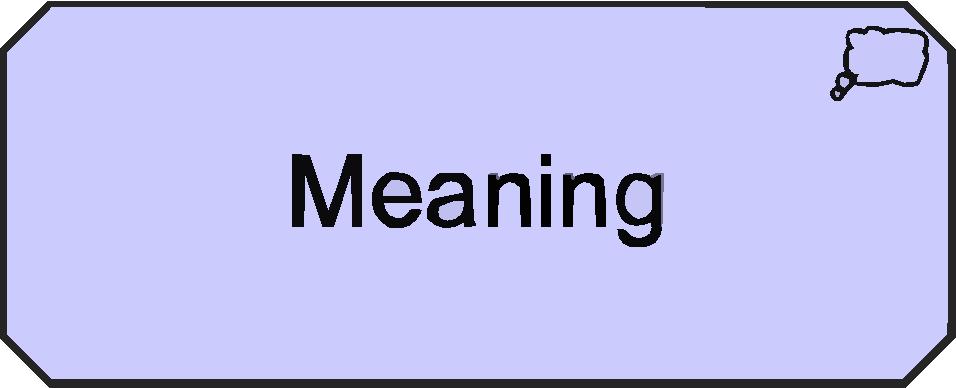
\includegraphics[width=1\linewidth]{imgs/capa_motivacional/meaning1.pdf}
\end{center} &
\begin{center}
    
\includegraphics[width=0.5\linewidth]{imgs/capa_motivacional/meaning2.pdf}
\end{center}
    \\ \hline

    Valor &
    Representa el valor relativo, la utilidad o la importancia de un concepto. &
\begin{center}
    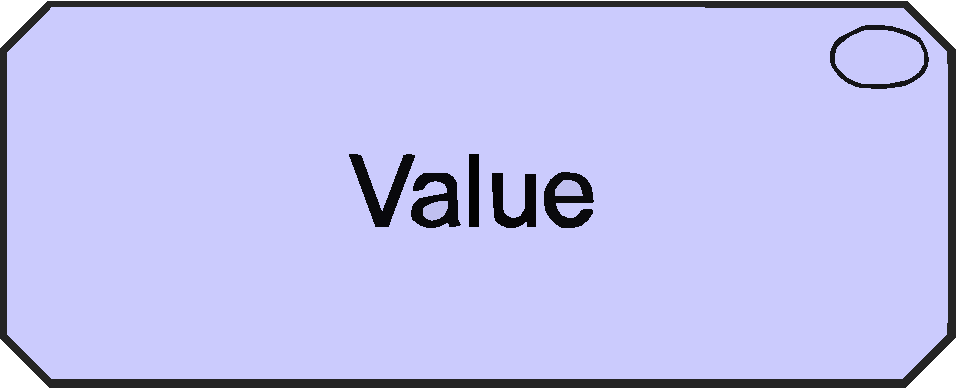
\includegraphics[width=1\linewidth]{imgs/capa_motivacional/value1.pdf}
\end{center} &
\begin{center}
    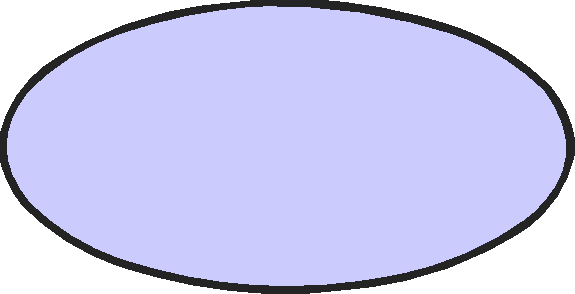
\includegraphics[width=0.5\linewidth]{imgs/capa_motivacional/value2.pdf}
\end{center}
    \\ \hline

\end{longtable}
